\documentclass[12pt]{article}
\usepackage{fancyhdr}
\usepackage{amsmath,amsfonts,enumerate}
\usepackage{color,graphicx}
\usepackage{tikz}
\usepackage{pgfplots}
\usepackage{listings}
\usepackage{algorithm}
\usepackage{algorithmic}
\usetikzlibrary{arrows,positioning,shapes,calc,matrix}
\pagestyle{fancy}
%%%%%%%%%%%%%%%%%%%%%%%%%%%%%%%%%%%%%%%%%%%%%%%%%
% Course customization based on Professor's teaching
%%%%%%%%%%%%%%%%%%%%%%%%%%%%%%%%%%%%%%%%%%%%%%%%%
\newcommand{\masunitnumber}{CENG 403}
\newcommand{\examdate}{January 2025}
\newcommand{\academicyear}{2024-2025}
\newcommand{\semester}{I}
\newcommand{\coursename}{Deep Learning - CNN Design \& Transfer Learning}
\newcommand{\numberofhours}{3}
%%%%%%%%%%%%%%%%%%%%%%%%%%%%%%%%%%%%%%%%%%%%%%%%%
% CUSTOM SPACING COMMANDS FOR ANSWER SPACES
%%%%%%%%%%%%%%%%%%%%%%%%%%%%%%%%%%%%%%%%%%%%%%%%%
\newcommand{\answerspace}[1]{\vspace{#1}}
\newcommand{\questionspace}{\vspace{3cm}}        
\newcommand{\subquestionspace}{\vspace{2.5cm}}   
\newcommand{\shortanswer}{\vspace{2cm}}          
\newcommand{\mediumanswer}{\vspace{3cm}}         
\newcommand{\longanswer}{\vspace{4cm}}           
\newcommand{\journalspace}{\vspace{4.5cm}}       
\newcommand{\codespace}{\vspace{5cm}}            
%%%%%%%%%%%%%%%%%%%%%%%%%%%%%%%%%%%%%%%%%%%%%%%%%
% Header setup
%%%%%%%%%%%%%%%%%%%%%%%%%%%%%%%%%%%%%%%%%%%%%%%%%
\lhead{}
\rhead{}
\chead{{\bf MIDDLE EAST TECHNICAL UNIVERSITY}}
\lfoot{}
\rfoot{}
\cfoot{}
\begin{document}
\setlength{\headsep}{5truemm}
\setlength{\headheight}{14.5truemm}
\setlength{\voffset}{-0.45truein}
\renewcommand{\headrulewidth}{0.0pt}
\begin{center}
SEMESTER \semester\ EXAMINATION \academicyear
\end{center}
\begin{center}
{\bf \masunitnumber\ -- \coursename}
\end{center}
\vspace{20truemm}
\noindent \examdate\hspace{45truemm} TIME ALLOWED: \numberofhours\ HOURS
\vspace{19truemm}
\hrule
\vspace{19truemm}
\noindent\underline{INSTRUCTIONS TO CANDIDATES}
\vspace{8truemm}
%%%%%%%%%%%%%%%%%%%%%%%%%%%%%%%%%%%%%%%%%%%%%%%%%%%%%%
% Instructions based on professor's emphasis
%%%%%%%%%%%%%%%%%%%%%%%%%%%%%%%%%%%%%%%%%%%%%%%%%%%%%%
\begin{enumerate}
\item This examination paper contains {\bf SIX (6)} questions and comprises 
{\bf EIGHT (8)} printed pages.
\item Answer all questions. 
The marks for each question are indicated at the beginning of each question.
\item Answer each question beginning on a {\bf FRESH} page of the answer book.
\item This {\bf IS NOT an OPEN BOOK} exam.
\item Show clear reasoning for your answers, especially intuitive explanations.
\item For architectural diagrams, draw clear components and explain design choices.
\item Connect concepts to examples discussed in lectures where relevant.
\item Explain the practical implications of design decisions.
\end{enumerate}
%%%%%%%%%%%%%%%%%%%%%%%%%%%%%%%%%%%%%%%%%%%%%%%%%
% New page for questions
%%%%%%%%%%%%%%%%%%%%%%%%%%%%%%%%%%%%%%%%%%%%%%%%%
\newpage
\lhead{}
\rhead{\masunitnumber}
\chead{}
\lfoot{}
\cfoot{\thepage}
\rfoot{}
\setlength{\footskip}{45pt}
%%%%%%%%%%%%%%%%%%%%%%%%%%%%%%%%%%%%%%%%%%%%%%%%%%
% EXAM QUESTIONS BASED ON PROFESSOR'S TEACHING
%%%%%%%%%%%%%%%%%%%%%%%%%%%%%%%%%%%%%%%%%%%%%%%%%%

\paragraph{Question 1. Position-Sensitive Convolution and Pooling}{\hfill (25 marks)}\\
Based on the professor's explanation: "Vanilla convolution a CNN with vanilla convolution does not perform really well on such tasks" for position estimation.

\begin{enumerate}[(a)]
    \item The professor introduced position-sensitive convolution for problems where "we want to estimate a single quantity that represents the position of the object." Explain why vanilla CNNs struggle with position estimation tasks and how adding "I coordinate and J coordinate for each pixel as additional channels" solves this problem. \hfill (8 marks)
    
    \mediumanswer
    
    \item Compare pooling operations as described by the professor. Explain his statement that "complex cells do something similar to what we call pooling" in relation to neocognitron, and why "taking the maximum of the values in the receptive field works really well for many problems." \hfill (10 marks)
    
    \mediumanswer
    
    \item Analyze pooling's impact on translation invariance. The professor explained that "if the input slightly moved to the right...the maximum value is still within the receptive field." Calculate the translation tolerance for a max pooling layer with receptive field 3×3 and stride 2. \hfill (7 marks)
    
    \shortanswer
\end{enumerate}

\newpage
\paragraph{Question 2. Global Average Pooling and Fully Connected Layers}{\hfill (22 marks)}\\
The professor emphasized that "fully connected layers introduce some issues" and presented global average pooling as a solution.

\begin{enumerate}[(a)]
    \item Explain the two main problems with fully connected layers at the end of CNNs as discussed by the professor: the parameter explosion issue and the fixed input size limitation. Why does global average pooling solve both problems? \hfill (10 marks)
    
    \mediumanswer
    
    \item The professor described how global average pooling creates specialization: "different channels correspond to different objects and...we have the confidence maps highlighting the shape of the object." Explain this specialization mechanism and why "one fully connected layer is sufficient" after global average pooling. \hfill (8 marks)
    
    \mediumanswer
    
    \item The professor mentioned that "for this to work properly...we need like a similar number of channels as number of objects." Analyze the implications when this condition is not met and how the network can still "entangle" multiple objects through the policy layer. \hfill (4 marks)
    
    \shortanswer
\end{enumerate}

\newpage
\paragraph{Question 3. Fully Convolutional Networks}{\hfill (20 marks)}\\
Based on the professor's explanation: "Fully connected layers can be converted to convolution" for handling variable input sizes.

\begin{enumerate}[(a)]
    \item Describe the professor's method for converting fully connected layers to convolutional layers. Explain how "one neuron with full connectivity to its input layer" can be viewed as "a filter" and why this enables processing of higher resolution inputs. \hfill (8 marks)
    
    \mediumanswer
    
    \item The professor showed that converting FC layers to convolution produces "prediction maps" instead of single class probabilities. For a network trained on 224×224 images with 10 classes, describe what happens when you input a 448×448 image after FC-to-conv conversion. \hfill (8 marks)
    
    \mediumanswer
    
    \item According to the professor, "segmentation is a good example problem for this." Explain how fully convolutional networks enable pixel-level predictions by "sliding the whole network over the input." \hfill (4 marks)
    
    \shortanswer
\end{enumerate}

\newpage
\paragraph{Question 4. CNN Architecture Design Principles}{\hfill (25 marks)}\\
The professor provided a "simple blueprint" for CNN design and discussed experimental findings on architecture choices.

\begin{enumerate}[(a)]
    \item Reproduce the professor's CNN architecture blueprint showing the sequence: "convolution convolution is followed by some nonlinearity...this can be repeated...pooling...fully connected layers." Explain why this template is widely used. \hfill (8 marks)
    
    \begin{center}
    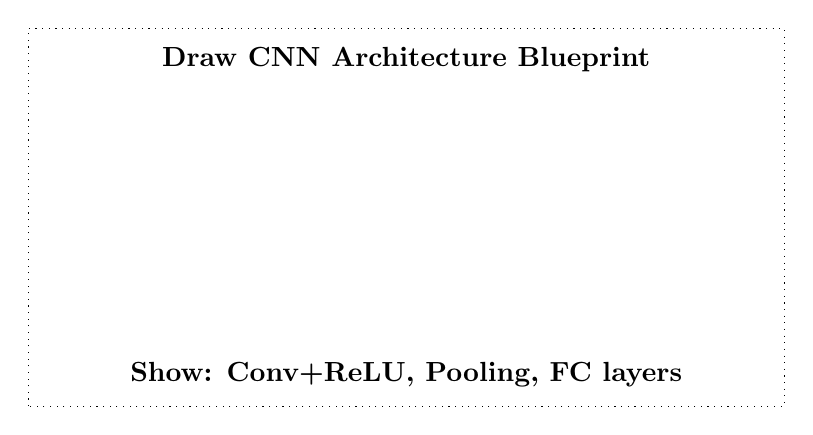
\begin{tikzpicture}[scale=0.8]
        % Space for CNN architecture blueprint
        \draw[dotted] (0,0) rectangle (12,6);
        \node at (6,5.5) {\textbf{Draw CNN Architecture Blueprint}};
        \node at (6,0.5) {\textbf{Show: Conv+ReLU, Pooling, FC layers}};
    \end{tikzpicture}
    \end{center}
    
    \shortanswer
    
    \item The professor discussed experimental findings: "deeper networks with smaller filters provided better results" and "depth is really critical." Explain why small filter size + deep network outperforms large filter size + shallow network, even when "one neuron in the top layer can cover the whole input range." \hfill (10 marks)
    
    \mediumanswer
    
    \item Analyze the professor's memory management strategy: "we will try to reduce dimensionality very quickly in the earlier parts of the network...information is redundant in the earlier layers." Explain why this approach works and give an example using AlexNet's "stride of four which reduces dimensionality by a factor of four." \hfill (7 marks)
    
    \mediumanswer
\end{enumerate}

\newpage
\paragraph{Question 5. Transfer Learning Strategies}{\hfill (28 marks)}\\
The professor explained: "We are not going to design something from scratch because it is very time consuming...we will take an existing CNN and adapt that CNN to our problem."

\begin{enumerate}[(a)]
    \item Describe the professor's four transfer learning scenarios based on problem similarity and data size. For each scenario, specify whether to freeze/fine-tune parameters and explain the reasoning: \hfill (16 marks)
    \begin{itemize}
        \item Similar problems + small data
        \item Similar problems + large data  
        \item Different problems + small data
        \item Different problems + large data
    \end{itemize}
    
    \journalspace
    
    \item The professor emphasized that "earlier parts are very generic problem independent" while "later parts are problem dependent they are specific to the problem." Explain this concept using the visualization evidence he referenced and how it guides transfer learning decisions. \hfill (8 marks)
    
    \mediumanswer
    
    \item According to the professor, when fine-tuning "you need to be careful with your learning rate...you can easily disrupt the learned rates." Explain why learning rate is critical in transfer learning and what happens if it's set too high. \hfill (4 marks)
    
    \shortanswer
\end{enumerate}

\newpage
\paragraph{Question 6. CNN Visualization and Interpretation}{\hfill (30 marks)}\\
The professor introduced multiple visualization techniques: "Understanding predictions why it makes those predictions is important."

\begin{enumerate}[(a)]
    \item Describe three visualization methods explained by the professor: activation visualization, weight visualization, and finding "images that maximize a neuron." For each method, explain what patterns indicate proper network functioning vs. problems. \hfill (12 marks)
    
    \longanswer
    
    \item The professor explained occlusion-based analysis: "We can slide an occlusion window over the whole input...this would indicate us whether this window is important for predicting that class or not." Explain how this method detects memorization vs. proper learning. \hfill (8 marks)
    
    \mediumanswer
    
    \item Implement the professor's gradient-based saliency map approach: "If we were to assume that we can approximate the whole CNN as if it was a linear model and we take the gradient...with respect to the input." Explain the mathematical foundation and why this "highlights which parts of the input are important for a problem." \hfill (10 marks)
    
    \mediumanswer
\end{enumerate}

\vfill
\begin{center}{\bf END OF PAPER}\end{center>
\end{document>